% Document class and font size
\documentclass[a4paper,10pt]{extarticle}

% Packages
\usepackage[utf8]{inputenc} % For input encoding
\usepackage{geometry} % For page margins
\geometry{a4paper, left=1.5cm, right=1.5cm, top=1.5cm, bottom=1.5cm} % Set paper size and margins
\usepackage{titlesec} % For section title formatting
\usepackage{enumitem} % For itemized list formatting
\usepackage{hyperref} % For hyperlinks
\usepackage{kotex}
\usepackage{graphicx}
\usepackage{array}
\usepackage{longtable}
\usepackage{tasks}
\usepackage{multirow}
\usepackage{tabularx, booktabs}
\usepackage{enumitem}
% Formatting
\setlist{noitemsep} % Removes item separation
\titleformat{\section}{\large\bfseries}{\thesection}{1em}{}[\titlerule] % Section title format
\titlespacing*{\section}{0pt}{\baselineskip}{\baselineskip} % Section title spacing
\graphicspath{{pictures}}

% Begin document
\begin{document}
% Global enumerate & itemize setting
\setlist{itemsep=0.05cm,labelindent=0.3cm,labelsep=0.3cm,leftmargin=*}
\setitemize{itemsep=0.02cm,labelindent=0.15cm,labelsep=0.3cm,leftmargin=*}
\renewcommand*{\arraystretch}{1.5}

% Disable page numbers
\pagestyle{empty}
% Enable page numbers
% \pagenumbering{arabic}

% Header
\begin{center}
	{\huge \textsc{Edward Hyeonbeen Lee}}
\end{center}

% \vspace*{-0.7cm}
\begin{center}
	\href{mailto:edward.hyeonbeen.lee@gmail.com}{edward.hyeonbeen.lee@gmail.com} $\bullet$ \href{https://github.com/leehyeonbeen}{GitHub (@leehyeonbeen)} $\bullet$ \href{https://scholar.google.com/citations?user=TiduRxoAAAAJ}{Google Scholar}
\end{center}

% \begin{center}
% 	\begin{table}[h!]
% 		\begin{tabularx}{\textwidth}{*3{>{\centering\arraybackslash}X}} % One left-aligned column, three equally spaced and centered columns
% 			\href{mailto:edward.hyeonbeen.lee@gmail.com}{edward.hyeonbeen.lee@gmail.com} $\bullet$ & \href{https://github.com/leehyeonbeen}{github.com/leehyeonbeen} $\bullet$ & \href{https://scholar.google.com/citations?user=TiduRxoAAAAJ}{Google Scholar}\\
%     \end{tabularx}
% 		% \begin{tabularx}{\textwidth}{*3 {>{\centering\arraybackslash}X}}
% 			% \href{mailto:edward.hyeonbeen.lee@gmail.com}{edward.hyeonbeen.lee@gmail.com} $\bullet$ & \href{https://github.com/leehyeonbeen}{github.com/leehyeonbeen} $\bullet$ & \href{https://scholar.google.com/citations?user=TiduRxoAAAAJ}{Google Scholar}
% 		% \end{tabularx}
% 	\end{table}
% \end{center}
% \vspace*{-1.2cm}


% \begin{minipage}{\textwidth}

% \begin{minipage}{0.1\textwidth}
% 	\begin{flushleft}
% 		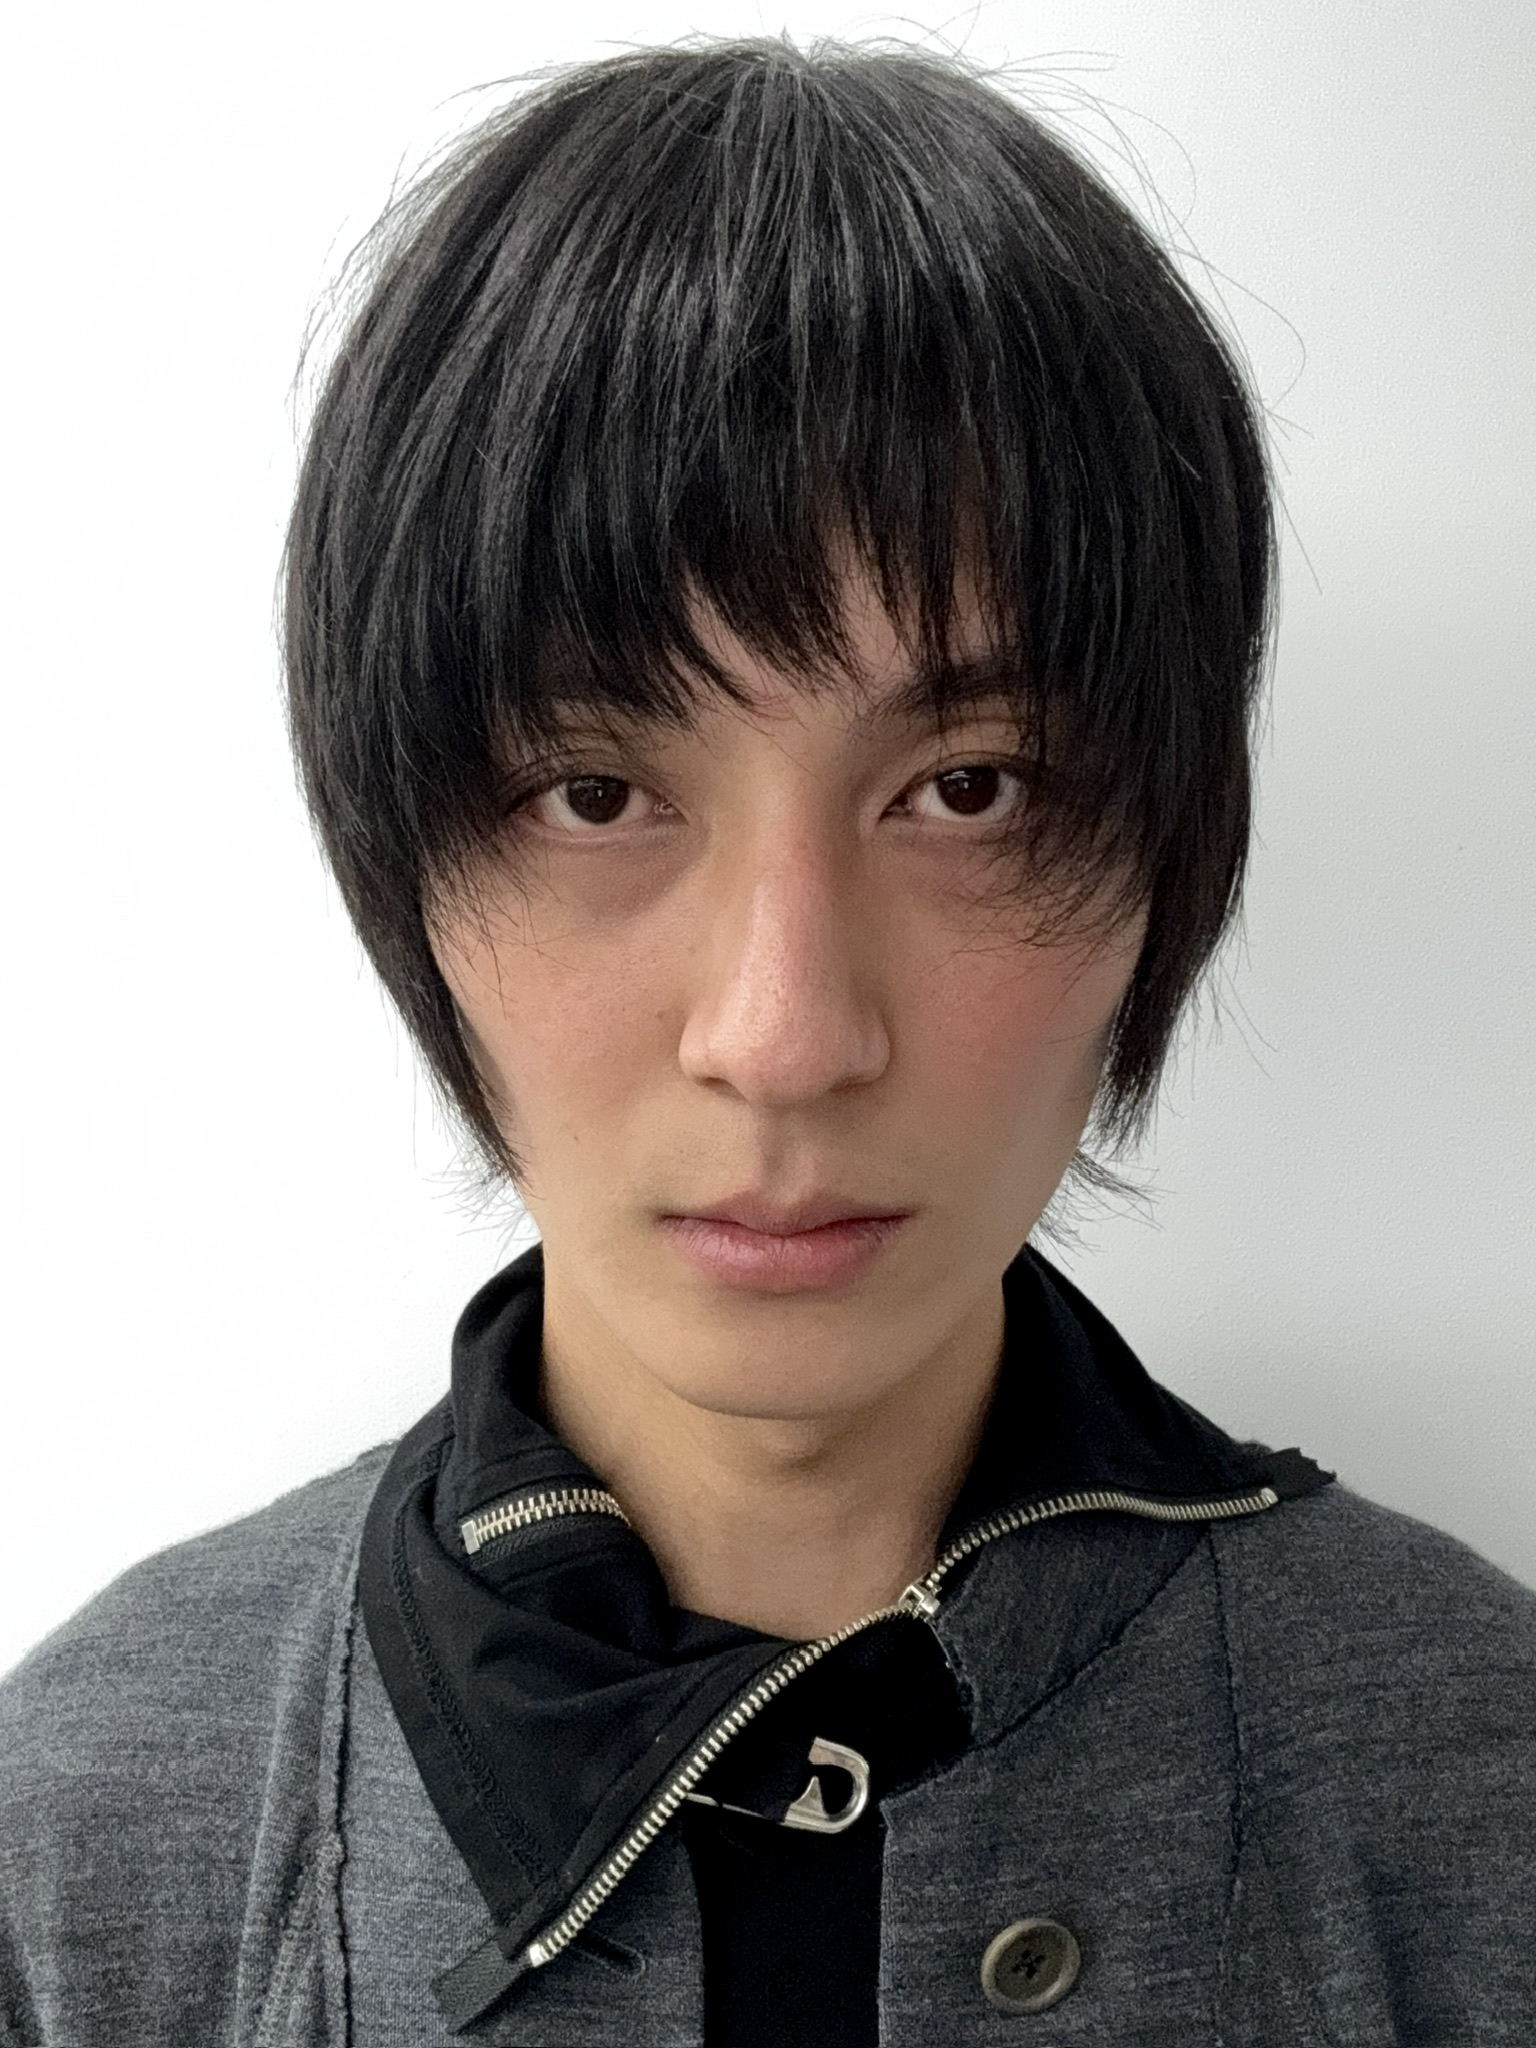
\includegraphics[height=3.5cm]{photo_dlicense.jpeg}
% 	\end{flushleft}
% \end{minipage}
% \hfill
% \begin{minipage}{0.7\textwidth}
% 	\begin{flushright}
% 		{\Huge Edward Hyeonbeen Lee} % Name
% 		\newline\newline
% 		\begin{tabular}{rl}
% 			\textbf{Mobile: }         & \href{tel:+82-10-6236-4693}{+82-10-6236-4693}                                                                 \\
% 			\textbf{EMail: }          & \href{mailto:edward.hyeonbeen.lee@gmail.com}{edward.hyeonbeen.lee@gmail.com}                                  \\
% 			\textbf{GitHub: }         & \href{https://github.com/leehyeonbeen}{github.com/leehyeonbeen}                                               \\
% 			% \textbf{Instagram: } & \href{https://www.instagram.com/leehyeonbeen}{@leehyeonbeen}                                         \\
% 			\textbf{LinkedIn: }       & \href{https://www.linkedin.com/in/hyeonbeen-lee-239500286/}{linkedin.com/in/hyeonbeen-lee-239500286}          \\
% 			\textbf{Google Scholar: } & \href{https://scholar.google.com/citations?user=TiduRxoAAAAJ}{scholar.google.com/citations?user=TiduRxoAAAAJ} \\
% 		\end{tabular}
% 		% \end{center}
% 	\end{flushright}

% \end{minipage}
% % \end{minipage}

% Personal Information Section
% \newcolumntype{L}{>{\raggedright\arraybackslash}m{3.5cm}}
% \newcolumntype{R}{>{\centering\arraybackslash\small}m{4cm}}
% \renewcommand*{\arraystretch}{1.4}
% \noindent
% \section*{PERSONAL INFORMATION}
% \begin{center}
% 	\vspace*{-0.8cm}
% 	\noindent
% 	\begin{longtable}{LRLRLR}
% 		\textbf{Legal Name:}                        & Hyeonbeen Lee                                        & \textbf{Date of birth:} & July 4th, 1996                                   \\
% 		\hline
% 		\textbf{Nationality:}                       & Republic of Korea (South)                            & \textbf{Address:}       & Hoenamu-ro 39gil, Yongsan-gu, Seoul, South Korea \\
% 		\hline
% 		\multirow{3}{*}{\textbf{Military service:}} & \multirow{3}{*}{\shortstack[c]{Honorably discharged,                                                                              \\ Marine Corps Sergeant \\{\small (May 2017$\sim$Feb. 2019)}}} & \multirow{3}{*}{\textbf{Research interest:}} & Robot learning\\ &&& Sensor fusion \\ &&&Sequential decision        \\
% 		\hline
% 	\end{longtable}
% \end{center}

\section*{RESEARCH INTEREST}
 \textbf{Robot learning, Sequential modeling, Robust autonomy, Multimodal perception, Interpretable AI}
% My works so far focus on accurate modeling of dynamic responses in contact-rich scenarios, which was a joyful journey with motivation. I desire to build a reliable robot intelligence that can robustly handle complex real-world interactions.
% \vspace*{-0.5cm}


% Education Section
\section*{EDUCATION}
\noindent
\textbf{Kyung Hee University} \hfill Mar. 2022 | Feb. 2024\\ % University name and location
M.S. in Mechanical Engineering (Advisor: Jin-gyun Kim) \hfill GPA: 3.93/4.0\\ % M.S. 3.93/4.0, 4.10/4.3, 4.33/4.5
% Thesis: \textit{{\small `Composite neural network with differential propagation}}\\
% \hspace*{1.3cm}\textit{\small{for modeling impulsive nonlinear dynamic systems'}}\\
\textbf{Kyung Hee University} \hfill Mar. 2015 | Feb. 2022\\ % University name and location
B.S. in Mechanical Engineering (Advisor: Jin-gyun Kim, Shin-kyu Jeong)\hfill GPA: 3.52/4.0 % B.S. Overall 3.52/4.0 ,3.599/4.3, 3.84/4.5
% Degree and GPA
% Thesis: \textit{{\small `Data-driven aerodynamic coefficient prediction using}} \hfill \textbf{GPA(Major): 3.51/4.0}\\  % B.S. Major 3.51/4.0, 3.573/4.3, ,3.87/4.5 
% \hspace*{1.3cm}\textit{{\small deep neural
% network and PARSEC airfoil parameterization'}} \\
% \textbf{Banpo High School}, Science-specialized Track \hfill Mar. 2012 | Feb. 2015

% Experience Section
\section*{PUBLICATIONS}
\begin{enumerate}[leftmargin=.5cm]
	\item \textbf{H. Lee}, M. Jung, J.G. Kim. (2025), “Forecasting high-frequency robot joint forces in contact-rich manipulation via short-time stationarity and neural frequency filters”, \textsl{Manuscript in preparation.}
	\item \href{https://www.sciencedirect.com/science/article/pii/S0021999123006733?casa_token=ARUkhI8XI8YAAAAA:wTzCIauJvSlonWw-J-SlAFqPX6NZRQS-qBX59l4YN5O3caEppoglU0duVmMkZYf4nWYd7tm_D_E}{\textbf{H. Lee}, S. Han, H.S. Choi, J.G. Kim (2024), “cNN-DP: Composite neural network with differential propagation for impulsive nonlinear dynamics”, \textit{Journal of Computational Physics (Q1, JCR-IF Top 4.5\% in Physics, Mathematical)}, 112578.}
	      % \item \href{https://easychair.org/publications/preprint/WkF3}{J.H. Han, J.B. Han, S.S. Kim, M.H. Kim, Y.H. Kim, \textbf{H. Lee}, J.G. Kim, T.K. Yeu. (2024), ``Digital twin model of underwater construction robot for real-time grinding simulation", \textit{7th International Conference on Multibody System Dynamics}.}
	\item \href{https://www.google.com/url?sa=t&rct=j&q=&esrc=s&source=web&cd=&cad=rja&uact=8&ved=2ahUKEwij36zWpNKCAxXMMEQIHSBfBMUQFnoECBEQAQ&url=https%3A%2F%2Fwww.sciencedirect.com%2Fscience%2Farticle%2Fpii%2FS1738573323003492&usg=AOvVaw1zj_G3k5c77uhMNnmu0EEC&opi=89978449}{S. Han, G.E. Jeong, \textbf{H. Lee}, W.S. Choi, J.G. Kim (2023), “Multi-body dynamics model for spent nuclear fuel transportation system under normal transport test conditions”, \textit{Nuclear Engineering and Technology (Q1, JCR-IF Top 3.5\% in Nuclear Science \& Technology)}, 55(11), 4125-4133.}
\end{enumerate}


\section*{RESEARCH EXPERIENCE}
% \setitemize{itemsep=0cm}
\noindent\textbf{Kyung Hee University} \hfill Postgraduate Researcher\\
Modeling \& Simulation Lab., advised by \textsl{Jin-gyun Kim} \hfill Mar. 2024 | Present\\
\vspace*{-0.25cm}\\
\begin{minipage}{0.75\textwidth}
	\small
	\begin{itemize}
		\item Developing a generalized framework for forecasting high-frequency force measurements of robot in contact-rich manipulation scenarios.
	\end{itemize}
\end{minipage}\\

% \noindent\textbf{Freelance AI developer} \hfill Freelancer\\
% --- \hfill Mar. 2024 | Present\\
% \hspace*{0.46cm}

\noindent\textbf{KAIST Graduate School of AI} \hfill Pre-Ph.D Research Intern\\
Cognitive Learning for Vision \& Robotics Lab., advised by \textsl{Joseph J. Lim} \hfill Sep. 2023 | Dec. 2023\\
\vspace*{-0.25cm}\\
\begin{minipage}{0.75\textwidth}
	\small
	\begin{itemize}
		\item Investigated skill-based reinforcement learning and skill prior extraction methodologies for learning-based robot control.
	\end{itemize}
\end{minipage}\\


\noindent\textbf{Kyung Hee University} \hfill Master Student\\
Modeling \& Simulation Lab., advised by \textsl{Jin-gyun Kim} \hfill Mar. 2022 | Feb. 2024\\
\vspace*{-0.25cm}\\
\begin{minipage}{0.75\textwidth}
	\small
	\begin{itemize}
		\item Led the development of a novel composite neural network (cNN-DP) for modeling impulsive nonlinear dynamics, resulting in a first-author publication in \textit{Journal of Computational Physics}.
		\item Executed and secured a national research grant by designing a deep generative forecasting model to predict reaction forces of underwater excavation robot.
		\item Contributed to a government-funded project by developing a DNN-based surrogate model for multi-body dynamics, leading to a co-authored publication in \textit{Nuclear Engineering and Technology}.
		\item Implemented and analyzed deep time-series and image models from scratch to expand the works for the real-world, multi-modal robotic systems.
	\end{itemize}
\end{minipage}\\

\vspace*{0.1cm}
\noindent\textbf{Kyung Hee University} \hfill Undergraduate Research Intern\\
Modeling \& Simulation Lab., advised by \textsl{Jin-gyun Kim} \hfill Jan. 2021 | Feb. 2022\\
\vspace*{-0.25cm}
\begin{minipage}{0.75\textwidth}
	\small
	\begin{itemize}
		\item Investigated data-driven methods for flexible multi-body dynamics.
	\end{itemize}
\end{minipage}\\
\vspace*{-0.2cm}





% \textbf{Pre-Ph.D Research Intern} \hfill Sep. 2023 | Dec. 2023\\
% Cognitive Learning for Vision \& Robotics Lab., Graduate School of AI, KAIST \hfill \\
% --- \textsl{Skill-based reinforcement learning, Skill prior extraction}\\
% \textbf{Undergraduate Research Intern} \hfill Jan. 2021 | Feb. 2022\\
% Modeling \& Simulation Lab., Dept. of Mechanical Eng., Kyung Hee University\\
% --- \textsl{Data-driven flexible multi-body dynamics, Composite neural network}

% \section*{CAREER}
% \noindent
% \textbf{8DIVISION}, Flagship Store Staff \hfill Feb. 2024 | Present
% \begin{itemize}
% 	\item Global fashion sales
% 	\item \textbf{Creative social media management (@8division, @8division$\_$journal)}
% 	\item Modeling and styling
% 	\item Robotic process automation using Python Selenium
% 	\item Sales analysis using Python dataprocessing libs
% \end{itemize}
% \textbf{Freelance model}\hfill May 2024 | Present
% \begin{itemize}
% 	\item \href{https://instagram.com/gyoureekim}{@gyoureekim} SS2025 fitting model for \href{https://instagram.com/londonfashionweek}{London Fashion Week}
% 	\item \href{https://instagram.com/san263_1}{@san263$\_$1} FW2024/SS2025 fitting model
% 	\item \href{https://instagram.com/8division}{@8division}, \href{https://instagram.com/8division_journal}{@8division$\_$journal} store fitting model
% 	\item \href{https://instagram.com/armed_dept}{@armed$\_$dept} FW2024 Lookbook
% 	\item Personal works with photographers: \href{https://instagram.com/chtewon}{@chtewon}, \href{https://instagram.com/wyw_kiki98}{@wyw$\_$kiki98}, \href{https://instagram.com/leeejaehoon}{@leeejaehoon}, \href{https://instagram.com/jngsnghun}{@jngsnghun}
% 	\item Magazines: \href{https://instagram.com/pap_magazine}{@pap$\_$magazine}, \href{https://instagram.com/prism.mag}{@prism.mag}
% \end{itemize}

% \section*{LANGUAGE}
% \subsection*{}
% \begin{itemize}
% 	\item English
% 	      \begin{itemize}
% 		      \item \textbf{Certification - New TEPS 513/600} (equivalent to 980/990 in ETS TOEIC)
% 		      \item \textbf{Certification - ACTFL OPI English AH(Advanced High)}
% 		      \item Expertised communication ability in native level
% 		      \item Rich communication experiences with global fashion creatives and designers
% 		      \item Published two papers for international science journals as first and co-author
% 		      \item Abundant experiences at international conference presentations, research meetings, and email communication in expert levels
% 	      \end{itemize}
% 	\item Japanese
% 	      \begin{itemize}
% 		      \item Able to speak daily-level conversations
% 		      \item Understands movies and TV shows in Japanese without subtitles
% 	      \end{itemize}
% \end{itemize}

% \subsection*{Global networking}
% Possesses communications, collaborations and socialization experiences with non-Korean fashion brands or influencers listed below:\\\\
% \noindent
% {\textbf{English speakers}}
% \begin{tasks}[style=itemize](3)
% 	\task Stefan Cooke \& Jake Burt
% 	\task SABUKARU
% 	\task Betsy Johnson
% 	\task RIER
% 	\task ThinkingMU
% 	\task FFFPostalService
% 	\task Luca Hamers
% 	\task GR10K
% 	\task Untitled Agency
% 	\task Bonnie \& Clyde
% 	\task SAMUTARO
% 	\task Hiking Patrol
% 	\task \_J.L-A.L\_
% 	\task Stockholm Surfboard Club
% 	\task JUS Stockholm
% 	\task DOUBLEU
% \end{tasks}

% \noindent
% {\textbf{Japanese speakers}}
% \begin{tasks}[style=itemize](3)
% 	\task Nepenthes
% 	\task KAMIYA
% 	\task PickYou
% 	\task COMOLI
% 	\task Ken Mitsuishi
% 	\task NorthWorks
% 	\task Huntism Tokyo
% 	\task OURs (YouTube)
% 	\task JunctionJP
% 	\task HLTVC
% \end{tasks}

\section*{AWARDS \& SCHOLARSHIPS}
\begin{itemize}
	\item \textbf{Excellent Paper Award} \hfill Korean Society of Mechanical Engineers, Aug. 2023 % No.2023-083, Aug 25 2023
	\item \textbf{RA Scholarship} \hfill Graduate School of Engineering, Kyung Hee University, Sep. 2022 | Feb. 2023 % Sep. 2022 | Sep. 2023
	      % \item \textbf{Dean's List} \hfill Dept. of Mechanical Eng., Kyung Hee University, 2021 % Mar. 
	\item \textbf{Academic Excellence Scholarship} \hfill Dept. of Mechanical Eng., Kyung Hee University, Mar. 2021 % Mar. 
\end{itemize}

% Experience Section
\section*{CONFERENCES}
\noindent
\newcolumntype{L}{>{\raggedright\arraybackslash}m{13cm}}
\newcolumntype{R}{>{\raggedright\arraybackslash}m{4cm}}
\vspace*{-.5cm}
\begin{longtable}{LR}
	\href{https://easychair.org/publications/preprint/WkF3}{J. Han, J.B. Han, S.S. Kim, M.H. Kim, Y.H. Kim, \textbf{H. Lee}, J.G. Kim, T.K. Yeu. “Digital twin model of underwater construction robot for real-time grinding simulation”, \textit{7th International Conference on Multibody System Dynamics}. }                                                                                                                                  & {Jun. 9 2024 \linebreak Madison, WI, USA}     \\
	\href{https://www.dbpia.co.kr/Journal/articleDetail?nodeId=NODE11709087}{\textbf{H. Lee}, J. Han, T. Yeo, J.G. Kim. “Real-time multi-horizon reaction force forecasting of ocean robot using interpretable Transformer”, \textit{Annual Conference, Korean Society of Mechanical Engineers} (Oral Presentation).}                                                                                                                            & {Nov. 1 2023 \linebreak Incheon, South Korea} \\
	\href{https://www.dbpia.co.kr/journal/articleDetail?nodeId=NODE11511050}{\textbf{H. Lee,} S. Han, H.S. Choi, J.G. Kim. “Meta-modeling of nonlinear impulsive dynamics using composite neural network model with differential propagation”, \textit{Conference on Engineering Reliability, Korean Society of Mechanical Engineers} (\textbf{Excellent Paper Award}, Oral Presentation). \textsl{Extended works from IMAC 2023 presentation.}} & {May 18 2023 \linebreak Busan, South Korea}   \\
	% \href{https://www.dbpia.co.kr/Journal/articleDetail?nodeId=NODE11527668}{\textbf{H. Lee,} S. Han, H.S. Choi, J.G. Kim. “Composite Neural Network with Differentiation Propagation for Modeling Nonlinear Impulsive Dynamics”, \textit{Conference on Dynamics and Control, Korean Society of Mechanical Engineers} (Oral Presentation)}.                                        & {Mar. 23 2023 \linebreak Jeju, South Korea}   \\
	\href{https://link.springer.com/chapter/10.1007/978-3-031-34946-1_21}{\textbf{H. Lee,} S. Han, H.S. Choi, J.G. Kim. “Composite neural network framework for modeling impulsive nonlinear dynamic responses”, \textit{41th International Modal Analysis Conference (IMAC)} (Oral Presentation).}                                                                                                                                              & {Feb. 16 2023 \linebreak  Austin, TX, USA}    \\
	\textbf{H. Lee}, J.G. Kim. “Development of multibody dynamics trailer model using normal transportation test data and DNN based surrogate model generation”, \textit{Fall conference, Korean Society for Noise and Vibration Engineering} (Oral Presentation).                                                                                                                                                                               & {Dec. 4 2022 \linebreak Jeju, South Korea}    \\
\end{longtable}


% Experience Section
\setlength{\itemsep}{10pt} % Set to 0 to remove space
\section*{PROJECTS}
\begin{itemize}
	\item Segment Anyone: Fine-tuned Segment-Anything-Model (SAM) for human-collaborative robots, Kyung Hee University Dept. of Artifical Intelligence. (\href{https://github.com/leehyeonbeen/segment-anything-fine-tuning}{github.com/leehyeonbeen/segment-anything-fine-tuning})

	\item Deep sequence-to-sequence models from scratch: From RNN to advanced Transformer variants, Personal project. (\href{https://github.com/leehyeonbeen/TimeSeriesSeq2Seq}{github.com/leehyeonbeen/TimeSeriesSeq2Seq})

	\item ROS SLAM one-shot setup for Apple Silicon devices, Personal project. (\href{https://github.com/leehyeonbeen/ROS-SLAM-AppleSilicon}{github.com/leehyeonbeen/ROS-SLAM-AppleSilicon})

	\item cNN-DP: Composite neural network with differential propagation for impulsive nonlinear dynamics, Modeling \& Simulation Lab. (\href{https://github.com/leehyeonbeen/cNN-DP}{github.com/leehyeonbeen/cNN-DP})

	\item RecurDyn Automation using Python, Modeling \& Simulation Lab. (\href{https://github.com/leehyeonbeen/RecurDynPython}{github.com/leehyeonbeen/RecurDynPython})
\end{itemize}
% \noindent
% \newcolumntype{L}{>{\raggedright\arraybackslash}m{13cm}}
% \newcolumntype{R}{>{\raggedright\arraybackslash}m{4cm}}
% \vspace*{-.6cm}
% \begin{longtable}{LR}
% 	% \underline{Ongoing:} Probabilistic-Deterministic Hybrid Fourier Networks for High-Frequency Sensor Dynamics
% 	% Deep-learning based reaction force and torque prediction model development for underwater ground cutting robot using experimental measurements and dynamic simulation data, Korea Research Institute of Ships and Ocean Engineering (KRISO). (\textit{Manuscript in preparation}) & {Mar. 2022 | Present}   \\

% 	% {Apr. 2024 | May. 2024} & Automatic products registration, 8DIVISION. (\href{github.com/leehyeonbeen/AfterCompany-AutoProductReg}{github.com/leehyeonbeen/AfterCompany-AutoProductReg})                                                                                                              \\

% 	$\bullet$ cNN-DP: Composite neural network with differential propagation for impulsive nonlinear dynamics, Modeling \& Simulation Lab. (\href{https://github.com/leehyeonbeen/cNN-DP}{github.com/leehyeonbeen/cNN-DP})                                                              & {Nov. 2021 | Jan. 2024} \\

% 	% Metamodel generation and evolution procedures for flexible multibody dynamics, FunctionBay Inc.                                                                                                                                                                            & {Sep. 2021 | Jan. 2024} \\

% 	$\bullet$ ROS SLAM setup package distribution for Apple Silicon devices, Personal project. (\href{https://github.com/leehyeonbeen/ROS-SLAM-AppleSilicon}{github.com/leehyeonbeen/ROS-SLAM-AppleSilicon})                                                                            & {Sep. 2023 | Oct. 2023} \\

% 	$\bullet$ Bottom-Up codes development of time series AI models: From RNN to advanced Transformers, Personal project. (\href{https://github.com/leehyeonbeen/TimeSeriesSeq2Seq}{github.com/leehyeonbeen/TimeSeriesSeq2Seq})                                                          & {Mar. 2022 | Aug. 2023} \\

% 	$\bullet$ Segment Anyone: Fine-tuned Segment-Anything-Model (SAM) for human-collaborative robots, Kyung Hee University Dept. of Artifical Intelligence. (\href{https://github.com/leehyeonbeen/segment-anything-fine-tuning}{github.com/leehyeonbeen/segment-anything-fine-tuning}) & {Mar. 2023 | Jun. 2023} \\

% 	$\bullet$ RecurDyn Automation using Python, Modeling \& Simulation Lab. (\href{https://github.com/leehyeonbeen/RecurDynPython}{github.com/leehyeonbeen/RecurDynPython})                                                                                                             & {Dec. 2022 | Jun. 2023} \\

% 	% Development of ground·sea transportation test simulation model using multibody dynamics and DNN-based metamodel, Korea Atomic Energy Research Institute (KAERI). (Codes under classification.)                                                                             & {Sep. 2021 | Oct. 2022} \\
% \end{longtable}

% % Experience Section
\section*{GRANTS}
\noindent
\newcolumntype{L}{>{\raggedright\arraybackslash}m{13cm}}
\newcolumntype{R}{>{\raggedright\arraybackslash}m{4cm}}
\vspace*{-.5cm}
\begin{longtable}{LR}
	Deep-learning based reaction force prediction of underwater excavation robot using experimental measurements and dynamic simulation, \textit{Korea Research Institute of Ships and Ocean Engineering (KRISO).} & {Mar. 2022 | Oct. 2024} \\

	Metamodel generation and evolution procedures for flexible multibody dynamics, \textit{FunctionBay Inc.}                                                                                                       & {Mar. 2021 | Feb. 2024} \\
	% {Apr. 2024 | May. 2024} & Automatic products registration, 8DIVISION. (\href{github.com/leehyeonbeen/AfterCompany-AutoProductReg}{github.com/leehyeonbeen/AfterCompany-AutoProductReg})                                                                                                              \\

	% 	% {Nov. 2021 | Jan. 2024} & cNN-DP: Composite neural network with differential propagation for impulsive nonlinear dynamics, Modeling \& Simulation Lab. (\href{https://github.com/leehyeonbeen/cNN-DP}{github.com/leehyeonbeen/cNN-DP})                                                               \\
	% 	Metamodel generation and evolution procedures for flexible multibody dynamics, \textit{FunctionBay Inc.}                                                                                                       & {Sep. 2021 | Jan. 2024} \\

	% 	% {Sep. 2023 | Oct. 2023} & ROS SLAM setup package distribution for Apple Silicon devices, Personal project. (\href{github.com/leehyeonbeen/ROS-SLAM-AppleSilicon}{github.com/leehyeonbeen/ROS-SLAM-AppleSilicon})                                                                                     \\

	% 	% {Mar. 2022 | Aug. 2023} & Bottom-Up codes development of time series AI models: From RNN to advanced Transformers. (\href{github.com/leehyeonbeen/TimeSeriesSeq2Seq}{github.com/leehyeonbeen/TimeSeriesSeq2Seq})                                                                                     \\

	% 	% {Mar. 2023 | Jun. 2023} & Segment Anyone: Fine-tuned Segment-Anything-Model (SAM) for human-collaborative robots, Kyung Hee University Dept. of Artifical Intelligence. (\href{https://github.com/leehyeonbeen/segment-anything-fine-tuning}{github.com/leehyeonbeen/segment-anything-fine-tuning})  \\
	% 	% {Dec. 2022 | Jun. 2023} & RecurDyn Automation using Python, Modeling \& Simulation Lab. (\href{https://github.com/leehyeonbeen/RecurDynPython}{github.com/leehyeonbeen/RecurDynPython})                                                                                                              \\
	Development of ground·sea transportation test simulation model using multi-body dynamics and DNN-based metamodel, \textit{Korea Atomic Energy Research Institute (KAERI).}                                     & {Sep. 2021 | Oct. 2022} \\
\end{longtable}

\section*{SKILLS}
\begin{itemize}
	\item \textbf{Programming Languages: }Python, MATLAB, C\#, C++, \LaTeX
	\item \textbf{ML and Data Analysis:} PyTorch, TensorBoard, Torchvision, OpenCV, Pillow, Pandas, SciPy, Seaborn
	\item \textbf{Tools and Systems: }Docker, Git, Linux, ROS, RecurDyn
	\item \textbf{Natural Languages: }Korean (native), English and Japanese (advanced proficiency)
	      %   \begin{itemize}
	      %       \item \textit{Expertised at handling \underline{sequential data and models}}
	      %   \end{itemize}
	      % \item \textbf{English: }Speaks at native level
	      % \item \textbf{Japanese: }Speaks at intermediate level
\end{itemize}

\section*{TEACHING \& MENTORSHIP}
\textbf{Research Mentor} \hfill Modeling \& Simulation Lab., Kyung Hee University\\
--- \textsl{Guiding a junior graduate student on time series analysis and modeling.} \hfill Mar. 2025 | Present\\ % Mar. 2022 | Jun. 2023
\textbf{Teaching Assistant, Multibody System Dynamics} \hfill Dept. of Mechanical Eng., Kyung Hee University\\
--- \textsl{Lectured on computational multi-body dynamics with  theoretical derivations.} \hfill Mar. 2022 | Jun. 2023 % Mar. 2022 | Jun. 2023

% Skills Section
% \section*{CERTIFICATES}
% \begin{itemize}
% 	\item \textbf{New TEPS:} 513/600 (equivalent to TOEIC 980/990) \hfill No.0111736, Valid, May 13 2023

% 	\item \textbf{ACTFL OPI English:} AH (Advanced High) \hfill 2A7617334333, Valid, Nov. 14 2023
% 	      % \item \textbf{RA Scholarship (80\% tuition)} \hfill Kyung Hee University, Sep. 01 2023
% 	      % \item \textbf{Exellence Paper Award} \hfill Korean Society of Mechanical Engineers, No.2023-083, Aug. 25 2023
% 	      % \item \textbf{RA Scholarship (80\% tuition)} \hfill Kyung Hee University, Mar. 01 2023
% 	      % \item \textbf{RA Scholarship (80\% tuition)} \hfill Kyung Hee University, Sep. 01 2022
% 	      % \item \textbf{행정조교 장학금} \hfill 경희대학교 대학원, 수혜년월: 2022.09 | 2024.02
% 	      % \item \textbf{Excellence Scholarship (Full tuition)} \hfill Kyung Hee University, Mar. 01 2021
% 	\item \textbf{TOEIC:} 925/990 \hfill No.605083, Expired, Nov. 25 2018
% \end{itemize}



% \textbf{Representative Administration Assistant} \hfill Dept. of Mechanical Eng., Kyung Hee University, Sep 2022 | Present\\
% \textbf{Multibody dynamics} \hfill Kyung Hee University, Mar 2022 | Jun 2023\\
% \noindent
% \newcolumntype{L}{>{\raggedright\arraybackslash}m{12cm}}
% \newcolumntype{R}{>{\raggedright\arraybackslash}m{5cm}}
% \vspace*{-.5cm}
% \begin{longtable}{LR}
% 	\textbf{Administration Assistant} & Dept. of Mechanical Eng., Kyung Hee University
% \end{longtable}
% Experience Section
% \section*{사회경험}
% \noindent
% \textbf{맥도날드 서울교대점} 고객응대, 주방보조, 계산 \hfill 2014.11 - 2015.02\\
% \textbf{육회한연어 수원영통점} 서빙, 주방보조, 계산 \hfill 2016.02 - 2016.06\\
% \textbf{슈펜 가로수길점} 외국인 고객응대, 물류창고정리 \hfill 2016.06 - 2016.09\\
% \textbf{오늘 와인한잔 수원역점} 서빙, 주방보조 \hfill 2016.09 - 2016.12\\
% \textbf{아이리스 BAR} 서빙, 주방보조, 고객응대 \hfill 2019.03 - 2019.06\\
% \textbf{대명GEC} 삼성전자 화성사업장 케이블 배선작업 \hfill 2019.07 - 2019.08\\
% \textbf{Seminar: IAS18 Workshop\&Tutorials} \hfill {\small Intl. Conference on Intelligent Autonomous Systems}, Jul 2023\\
% \textbf{Seminar: AI Summer School 2022} \hfill Korean Society of Mechanical Engineers, Aug 2022\\
% \textbf{Teaching Assistant (System Dynamics)} \hfill Modeling \& Simulation Lab, Mar 2022 - Jun 2023\\
% \textbf{Seminar: AI Summer School 2021} \hfill Korean Society of Mechanical Engineers, Aug 2021\\
% \textbf{Seminar: AI, Data Driven Models\&ML} \hfill {\small National Agency Finite Element Methods and Standard}, Apr 2021\\
% \textbf{Undergraduate Research Internship} \hfill Modeling \& Simulation Lab, Jan 2021 | Feb 2022\\
% \textbf{48th Student Council} \hfill Kyung Hee University College of Engineering, Feb 2019 | Jan 2020\\
% \textbf{R.O.K.-U.S. Combined Marine Corps Interpreter} \hfill 1st Marine Div., ROKMC, Sep 2017 | Feb 2019\\


% \section*{SEMINARS}
% \textbf{Intl. Conference on Intelligent Autonomous Systems} \hfill Workshops \& Tutorials, Jul. 2023\\
% \textbf{Korean Society of Mechanical Engineers} \hfill AI Summer Camp, Aug. 2022\\
% \textbf{Korean Society of Mechanical Engineers} \hfill AI Summer Camp, Aug. 2021\\
% \textbf{\small National Agency for Finite Element Methods and Standards} \hfill {Seminar on data-driven models}, Apr. 2021\\


% Experience Section
\section*{LEADERSHIP \& SERVICE}
% \textbf{Representative Administrative Assistant} \hfill Kyung Hee University, Sep 2022 | Present\\
% \textbf{Seminar: IAS18 Workshop \& Tutorials} \hfill {\small Intl. Conference on Intelligent Autonomous Systems}, Jul. 2023\\
% \textbf{Seminar: AI Summer School 2022} \hfill Korean Society of Mechanical Engineers, Aug. 2022\\
% \textbf{Teaching Assistant (System Dynamics)} \hfill Modeling \& Simulation Lab, Mar 2022 - Jun 2023\\
% \textbf{Seminar: AI Summer School 2021} \hfill Korean Society of Mechanical Engineers, Aug. 2021\\
% \textbf{Seminar: AI, Data Driven Models \& ML} \hfill {\small National Agency Finite Element Methods and Standard}, Apr. 2021\\
% \textbf{Fashion Model} \hfill East Casting Agency, Mar. 2024 | Present\\
\textbf{Lead Administrative Assistant} \hfill Dept. of Mechanical Engineering, Kyung Hee University, 2022 | 2024\\
% \null\hfill \\ % Sep. 2022 | Feb. 2024
\textbf{College of Engineering 48th Student Council} \hfill Kyung Hee University, Feb 2019 | Jan. 2020\\
% \null\hfill \\
\textbf{R.O.K.-U.S. Combined Marine Corps Interpreter} \hfill 1st Marine Div., ROKMC, Sep 2017 | Feb. 2019\\
% End document
\end{document}